\chapter{Implementation}

\begin{figure}
\begin{center}
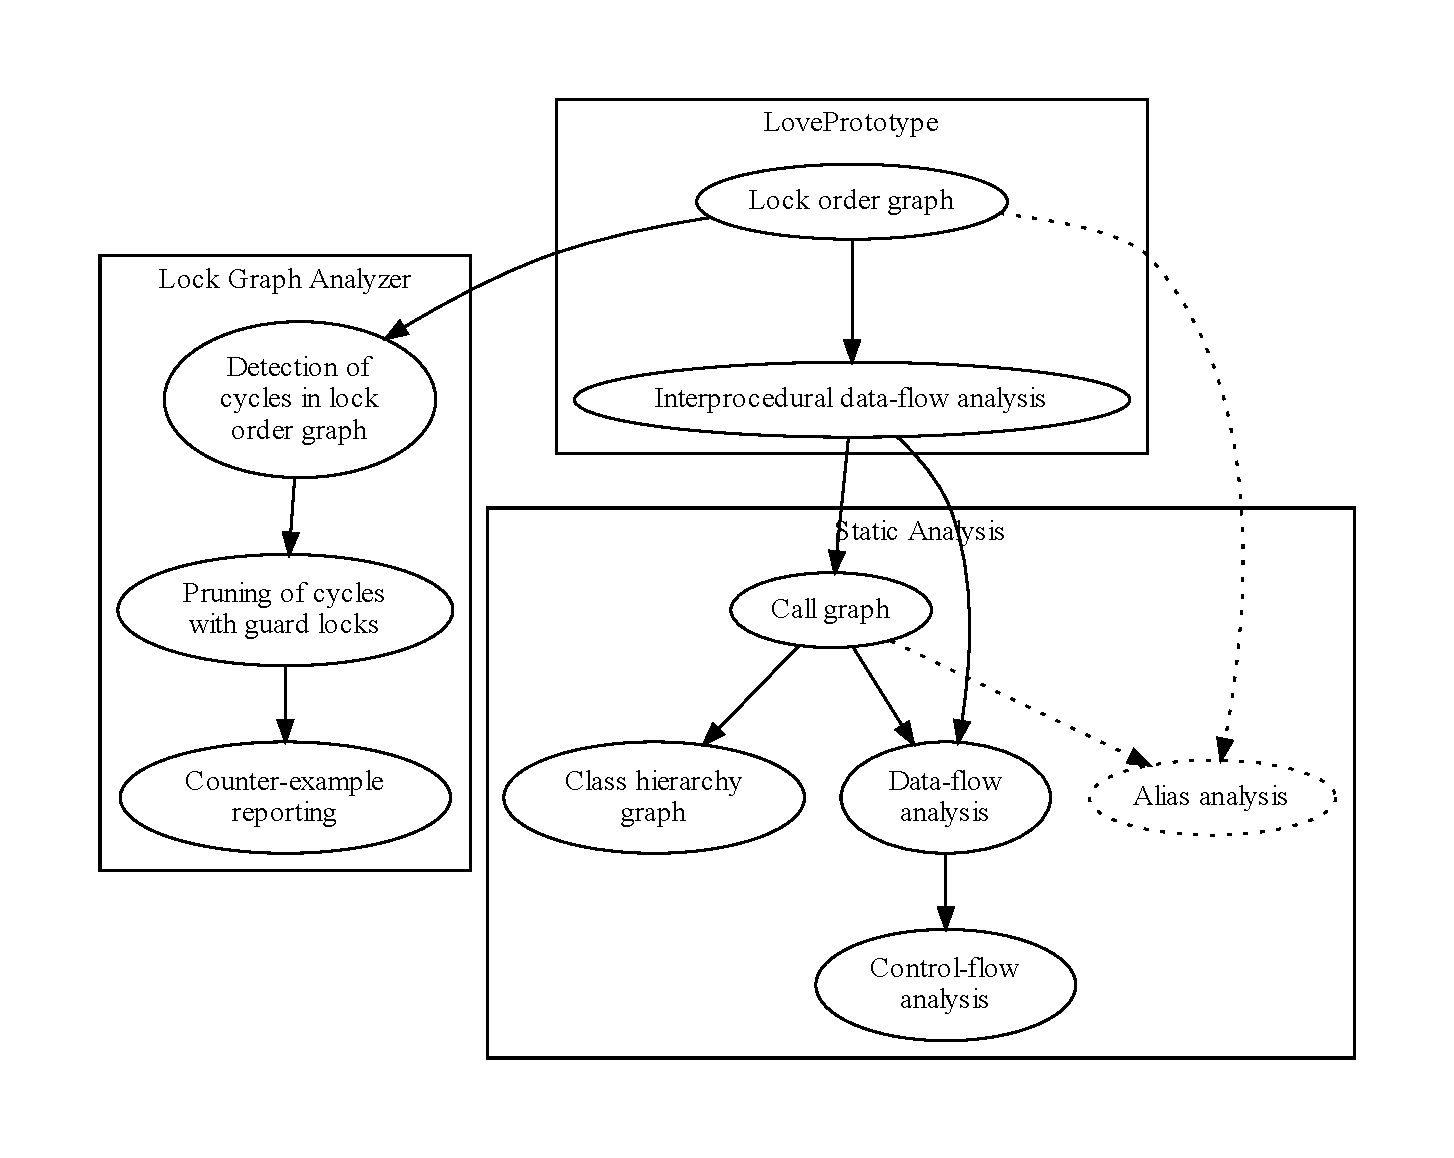
\includegraphics[scale=0.5]{Architecture.pdf}
\caption{High-level architecture of the tool}
\label{fig:architecture}
\end{center}
\end{figure}

The high-level architecture of the tool is shown on Figure ~\ref{fig:architecture}.

Mono.Cecil \citep{MonoCecil} library is used for manipulation of the program assemblies and their low-level structure and code in the intermediate language.

QuickGraph \citep{QuickGraph} library is used for manipulation of graphs. The library provides data structures for representing graphs and implements a wide variety of standard graph algorithms that operate on these data structures.

A library of common static analysis techniques is built on top of Mono.Cecil and QuickGraph libraries. It supplies a reusable implementation of class hierarchy extraction, control-flow analysis, data-flow analysis and call graph extraction.

On top of the static analysis library the \emph{LovePrototype} tool is built that constructs a call graph and then extracts the lock order graph using interprocedural data-flow analysis. The output of the tool is a lock order graph written to a file in GML (graph markup language) format.

\emph{Lock Graph Analyzer} tool is provided for analysis of the lock order graph. It takes the GML file as an input and searches the lock order graph for potential deadlocks and reports each of them into a separate DOT file. The DOT file contains the graph representing the lock order violation and accompanying information. It can be rendered using the GraphViz \citep{GraphViz} or MSAGL \citep{MsAgl} tools.

Additionally, several tools were developed to aid visualizing the graphs that are used during the analysis. Namely the \emph{GraphInspector} library, which provides a quick way of visually browsing through a graph by navigating through successors and predecessors of a highlighted vertex, and the \emph{GmlToSea} tool, which converts the standard GML format to an input suitable for the Walrus tool \citep{Walrus}.

\section{Static analysis library}

Control-flow graph can be constructed using the \texttt{ControlFlowGraph} object. The construction of the graph follows the algorithm described in Section 3. Exception flow is separated from the normal flow except for \texttt{finally} blocks, which are considered a part of the normal flow.

Data-flow analysis is implemented using a \texttt{DataFlowProblem} abstract class, which specifies the rules for data-flow analysis, such as a flow function, the initial state and the merge operator. The solution to the abstract problem can be computed using \texttt{WorkListSolver}, which takes a problem description and a control-flow graph as parameters and uses the work-list algorithm to compute the solution as either a summary state or in- and out- states for individual basic blocks. Initially, the work-list is populated with all vertices of the control-flow graph. A depth-first search is used to sort the vertices in order to minimize recomputation. Vertices that are not part any cycle are consequently sorted in topological order. The solver operates on regular vertices of the control-flow graph and doesn't traverse the exception handlers.

An abstract call graph concept is implemented. The abstraction allows switching between different call graph extraction algorithms as appropriate for the specific task without requiring a change to the call graph consumer.

A \texttt{ChaCallGraphBuilder} call graph builder implements the simple class-hierarchy based call graph extraction algorithm as described in Chapter 2. All reachable methods from a single entrypoint are analyzed and added to the call graph. Virtual method calls are resolved using the declared variable type and class hierarchy graph. Delegates are resolved by matching the delegate type. For example, each new EventHandler(FunctionX) call contributes an edge between EventHandler.Invoke and FunctionX.

\begin{figure}
\begin{center}
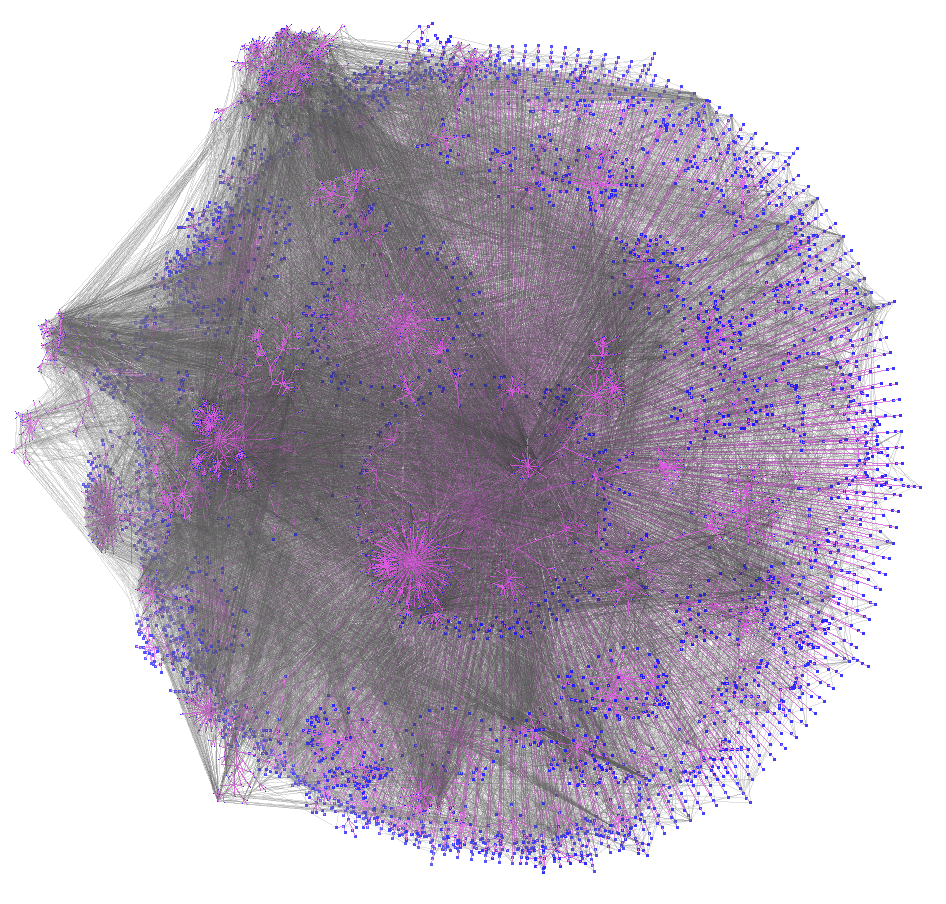
\includegraphics[scale=0.5]{CallGraph.png}
\end{center}
\caption{Computed rooted CHA call graph of a simple C\# test case program with three methods, as visualized by Walrus. The graph contains 7,177 vertices (methods) and 34,692 edges (calls), most of which come from the referenced Base Class Library. Moderately sized programs often have more than 100,000 vertices and 950,000 edges in the call graph, which is hard to visualize.}
\end{figure}

\section{LovePrototype tool}

The LovePrototype tool implements the design specified in Chapter 5. It uses the Static Analysis library for performing the intraprocedural data-flow computations and implements the interprocedural data-flow analysis using a work-list approach.

Additionally, the symbolic object aliasing behavior has several quirks that should be noted:
\begin{itemize*}
\item Fields and static fields marked as \texttt{readonly} are treated as unaliased. While this is unsound assumption it covers the most common locking pattern, where a \texttt{readonly} field is initialized with \texttt{new object()} and locked on.
\item Additional command line option \texttt{--noaliasing} is available that forces all fields to be treated as unaliased. This emulates the behavior of CSLint \citep{CSLint}.
\item Symbolic objects that represent method arguments keep reference to the original parameter they represent and thus two arguments of the same type are represented by distinct symbolic objects unlike the description in Chapter 5.
\end{itemize*} 

Command line option \texttt{--ignoresystemnamespace} is provided to suppress the analysis of all methods in the \texttt{System} namespace. This call graph is still built from all referenced classes and libraries and it is traversed even for methods belonging to the \texttt{System} namespace, locks are however not tracked.

Output of the tool is the call graph and lock graph in GML graph format with marked vertices that belong to the root set.

\begin{figure}[H]
\begin{center}
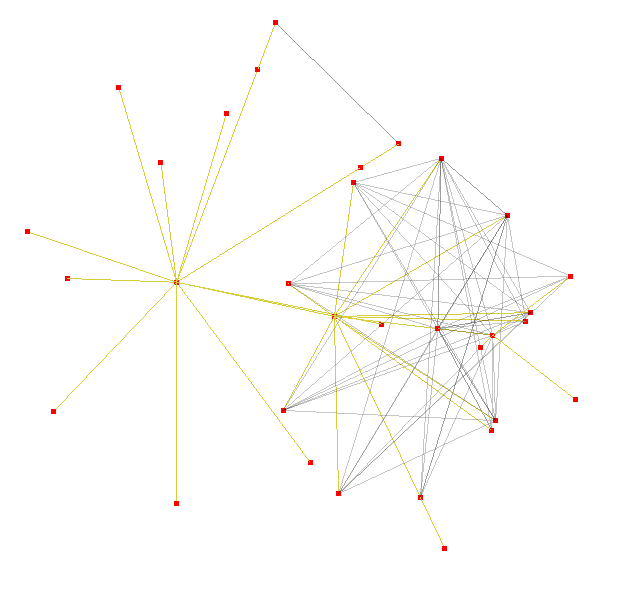
\includegraphics[scale=0.5]{LockGraph.png}
\end{center}
\caption{Computed lock graph of a simple C\# test case program with three methods, as visualized by Walrus. Tree edges are displayed in yellow and non-tree edges in gray.}
\end{figure}

\section{Lock Graph Analyzer}

The lock graph analyzer tool loads the lock order graph from the GML file produced by LovePrototype tool. It then uses depth-first search to classify all the graph edges as tree edges, back edges and forward / cross edges.

Back edges signify cycles in the graph. The tool searches specifically only for simple cycles with two edges. Thus lock order violations between more than two will not be found by this tool. These violations are rarely seen in practice and it would be trivial to extend the tool to find those cycles as well, however these cycles are often false positives caused by imprecise lock order graph construction.

Once a simple cycle is found all paths from the root locks (ie. locks that are roots of the lock order hierarchy in at least one thread) to the cycle edges are examined. These paths are built from the tree edges and forward / cross edges leading to the cycle, which implies that no other cycle is formed along these paths.

Dominance sets are computed for each vertex of the paths. If there is a common dominator between all vertices of the cycle, the dominator is considered a guard lock and the simple cycle is not considered to cause a deadlock.

Otherwise, the simple cycle is written to a DOT file for further examination by the programmer. The vertices correspond to the symbolic objects and edges are marked with the program point where the corresponding objects were acquired.

\begin{figure}
\begin{center}
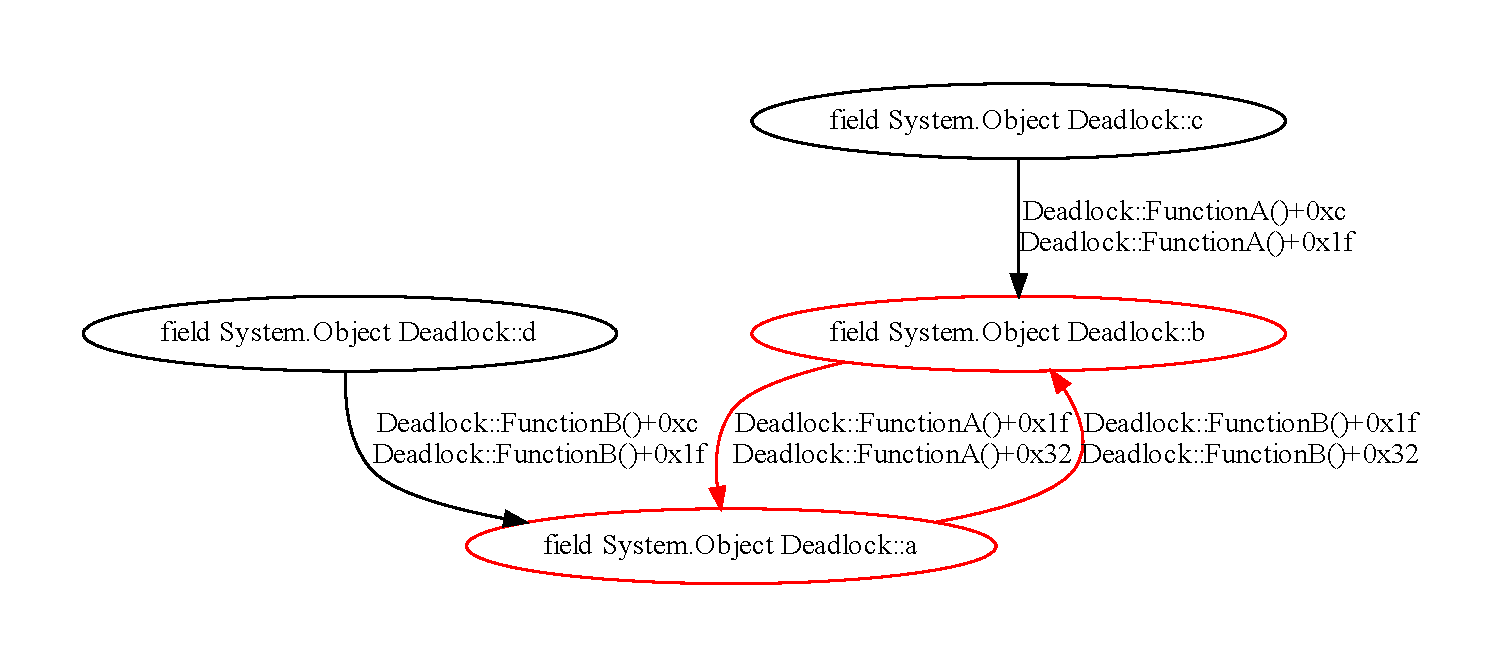
\includegraphics[scale=0.5]{LockGraphAnalyzerOutput.pdf}
\end{center}
\caption{Sample output of the Lock Graph Analyzer tool}
\end{figure}